\section{Selection of Lambda}

The additional term $\lambda \|\mathbf{\mathbf{X}}\|_2^2$ in the optimization
problem shown in equation~(\ref{eq:RRproblem}) has two effects on the solution:
shrinks the coefficients towards zero and improves the conditioning of the
problem.

Figure~\ref{fig:shrinks} shows a visual example of the shrinking of the
coefficients:

\begin{figure}[h!]
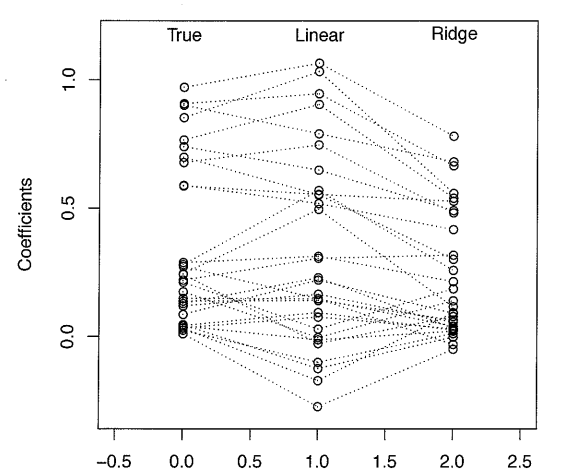
\includegraphics[width=0.5\linewidth]{plots/shrinks}
\caption{Shrink of regression coefficients}
\label{fig:shrinks}
\end{figure}




On the other hand, the effect of adding the term $\lambda \mathbb{I}$
to the matrix $\mathbf{A}^\top \mathbf{A}$
(equation~(\ref{eq:optsolRR})) improves its condition number since it
increases its diagonal values when $\lambda > 0 $.  The matrix
$\mathbf{A}^\top \mathbf{A}$ is symmetrical ($(\mathbf{A}^\top
\mathbf{A})^\top = \mathbf{A}^\top \mathbf{A}$) and therefore
diagonalizable.  If we know the eigenvalue decomposition of $\mathbf{A}
= \mathbf{U\Sigma V^\top}$, then:

\begin{eqnarray*}
\mathbf{A}^\top \mathbf{A}+\lambda \mathbb{I}&=&\mathbf{V\Sigma^2
V}^\top + \lambda \mathbf{V} \mathbf{V}^\top\\ &=&\mathbf{V}
(\mathbf{\Sigma}^2+\lambda\mathbb{I}) \mathbf{V}^\top \, ,
\end{eqnarray*}

\noindent where

\begin{equation*}
\mathbf{\Sigma}^2+\lambda\mathbb{I}=
\begin{bmatrix}
\sigma^2_1 + \lambda & \, & \, \\
\, & \sigma^2_2 +\lambda & \, \\
\, & \, & \ddots & \, \\
\, & \, & \, & \sigma^2_n +\lambda \, .
\end{bmatrix}
\end{equation*}

where $\sigma_1 \geq \sigma_2 \geq \dots \geq \sigma_n$.

Since the condition number of a matrix $\mathbf{A}$ is defined as:

\begin{equation*}
	\kappa = \|\mathbf{A}\| \|\mathbf{A}^{-1}\|
\end{equation*}

If matrix $\mathbf{A}$ is non-singular, its condition number can be
expressed in terms of its singular values. The effect of adding the
regularization term affects the condition number as follows:

\begin{eqnarray*}
\kappa_{ols} &=& \|\mathbf{A}\| \|\mathbf{A}^{-1}\|=\frac{\sigma_1}{\sigma_n} \\
\kappa_{ridge} &=& \|\mathbf{A}^\intercal \mathbf{A} + \lambda \mathbb{I}\| 
\|(\mathbf{A}^\intercal \mathbf{A} + \lambda \mathbb{I})^{-1}\|=\frac{\sigma_1+\lambda}{\sigma_n + \lambda} \,
\end{eqnarray*}

It is easy to see that the term $\lambda$ improves the condition number: 

\begin{equation*}
        \frac{\sigma_1+\lambda}{\sigma_n + \lambda} <
        \frac{\sigma_1}{\sigma_n} \,  \qquad \forall \quad \lambda > 0
\end{equation*}


However, $\lambda$ cannot be too large. Tipically $\lambda$ is small and its
magnitude depends on the matrix $\mathbf{A}$.

For rank deficient matrices we know that $\text{det}(\mathbf{A A^\top})=0$, adding the
term $\lambda \mathbb{I}$ we have that $\text{det}(\mathbf{A A^\top}+\lambda \mathbb{I}) =
p(\lambda)$ where $p(\lambda)$ is a polynomial of degree $n$ ($\mathbf{A}$ is
$m \times n$). The zeros of $p(\lambda)$ are discretes, so it can be represented
as:

\[
p(\lambda) =
\lambda(\lambda-\lambda_1)^{n_1}(\lambda-\lambda_2)^{n_2}\dots(\lambda-\lambda_s)^{n_s}
\]

\noindent where $n_1 + n_2 + \dots + n_s = n$.

This means that $\lambda$ must be small in order to ensure that $p(\lambda)$
does not vanish.

\subsection{The bias-variance tradeoff}

To determine parameter $\lambda$ is crucial for ridge regression since it could
reduce the expected prediction error by reducing variance considering a biased
estimator, this is called the bias-variance trafeoff. The prediction error is
obtained as:

\begin{equation}
 \label{eq:prederror}
E[(B-\hat{f}(\mathbf{X}))^2] = \sigma^2 + Bias(\hat{f}(\mathbf{X}))^2 + Var(\hat{f}(\mathbf{X}))
\end{equation}

\noindent where $\hat{f}(\mathbf{X})=\mathbf{AX}(\lambda)$ and
$f(\mathbf{X})=\mathbf{AX}$.


\textbf{Demo}\quad

\begin{eqnarray*}
E[(B-\hat{f}(\mathbf{X}))^2] & =&
E[(B-f(\mathbf{X})+f(\mathbf{X})-\hat{f}(\mathbf{X}))^2] \\
&=& E[(B-f(\mathbf{X}))^2] +
E[(f(\mathbf{X})-\hat{f}(\mathbf{X}))^2] + \dots \\
& &
2\cancelto{0}{E[B-f(\mathbf{X})]}E[f(\mathbf{X})-\hat{f}(\mathbf{X})] \\
&=& \sigma^2 + MSE(\hat{f}(\mathbf{X}))
\end{eqnarray*}

\noindent where 

\begin{eqnarray*}
    MSE(\hat{f}(\mathbf{X})) &=&
    E[f(\mathbf{X})-\hat{f}(\mathbf{X}))]^2 \\
    &=& E[f(\mathbf{X})-E[\hat{f}(\mathbf{X})] +
    E[\hat{f}(\mathbf{X})]-\hat{f}(\mathbf{X}))]^2 \\
    &=&  E[(f(\mathbf{X})-E[\hat{f}(\mathbf{X})])^2] +
      E[(\hat{f}(\mathbf{X})-E[\hat{f}(\mathbf{X})])^2] + \dots\\
    & & E[(f(\mathbf{X})-E[\hat{f}(\mathbf{X})])] 
    \cancelto{0}{E[(\hat{f}(\mathbf{X})-E[\hat{f}(\mathbf{X})])]} \\
    &=& Bias(\hat{f}(\mathbf{X}))^2 + Var(\hat{f}(\mathbf{X}))
\end{eqnarray*}

The bias of OLS is:

\begin{eqnarray*}
Bias(\hat{\mathbf{X}}) &=& E[\hat{\mathbf{X}}] - \mathbf{X} \\
&=& E[ (\mathbf{A}^\top \mathbf{A})^{-1}\mathbf{A}^\top \mathbf{B}] - \mathbf{X} \\
&=& E[ (\mathbf{A}^\top \mathbf{A})^{-1}\mathbf{A}^\top (\mathbf{AX})] - \mathbf{X}  \\
&=& \mathbf{X}  - \mathbf{X}  \\
&=&  0
\end{eqnarray*}


The bias of ridge regression when $\mathbf{A A^\top}$ is non-singular
can be obtained expressing ridge regression solution
$\mathbf{\lambda}$ in terms of OLS solution $\hat{\mathbf{X}}$:

\begin{eqnarray*}
\mathbf{X}(\lambda) &=&( \mathbf{A}^\top \mathbf{A} + \lambda \mathbb{I})^{-1}\mathbf{B} \\
&=& (\mathbb{I} + \lambda (\mathbf{A}^\top \mathbf{A})^{-1})^{-1} (\mathbf{A}^\top \mathbf{A})^{-1}\mathbf{A}^\top \mathbf{B} \\
&=&  (\mathbb{I} + \lambda (\mathbf{A}^\top \mathbf{A})^{-1})^{-1}  \hat{\mathbf{X}} \\
&=& \mathbf{W} \hat{\mathbf{X}} 
\end{eqnarray*}

\noindent where $\mathbf{W}  = (\mathbb{I} + \lambda (\mathbf{A}^\top
\mathbf{A})^{-1})^{-1}  $ it is defined for simplicity. Ridge
regression bias is then obtained as:

\begin{eqnarray*}
Bias(\mathbf{X}(\lambda)) &=& E[\mathbf{X}(\lambda)] - \mathbf{X} \\
&=& E[\mathbf{W}\hat{\mathbf{X}}] - \mathbf{X} \\
&=&  \mathbf{W} \mathbf{X} - \mathbf{X} \neq 0 
\end{eqnarray*}



The variance of OLS is:

\begin{equation*}
Var(\hat{\mathbf{X}}) = \sigma^2 (\mathbf{A}^\top \mathbf{A} )^{-1}
\end{equation*}

\noindent and the variance of ridge regression is:

\begin{eqnarray*}
Var(\mathbf{X}(\lambda)) &=& Var(\mathbf{W}\hat{\mathbf{X}}) \\ 
&=& \mathbf{W}Var(\hat{\mathbf{X}})\mathbf{W}^\top \\
&=& \sigma^2 \mathbf{W}(\mathbf{A}^\top \mathbf{A} )^{-1}\mathbf{W}^\top
\end{eqnarray*}


\begin{figure}[h!]
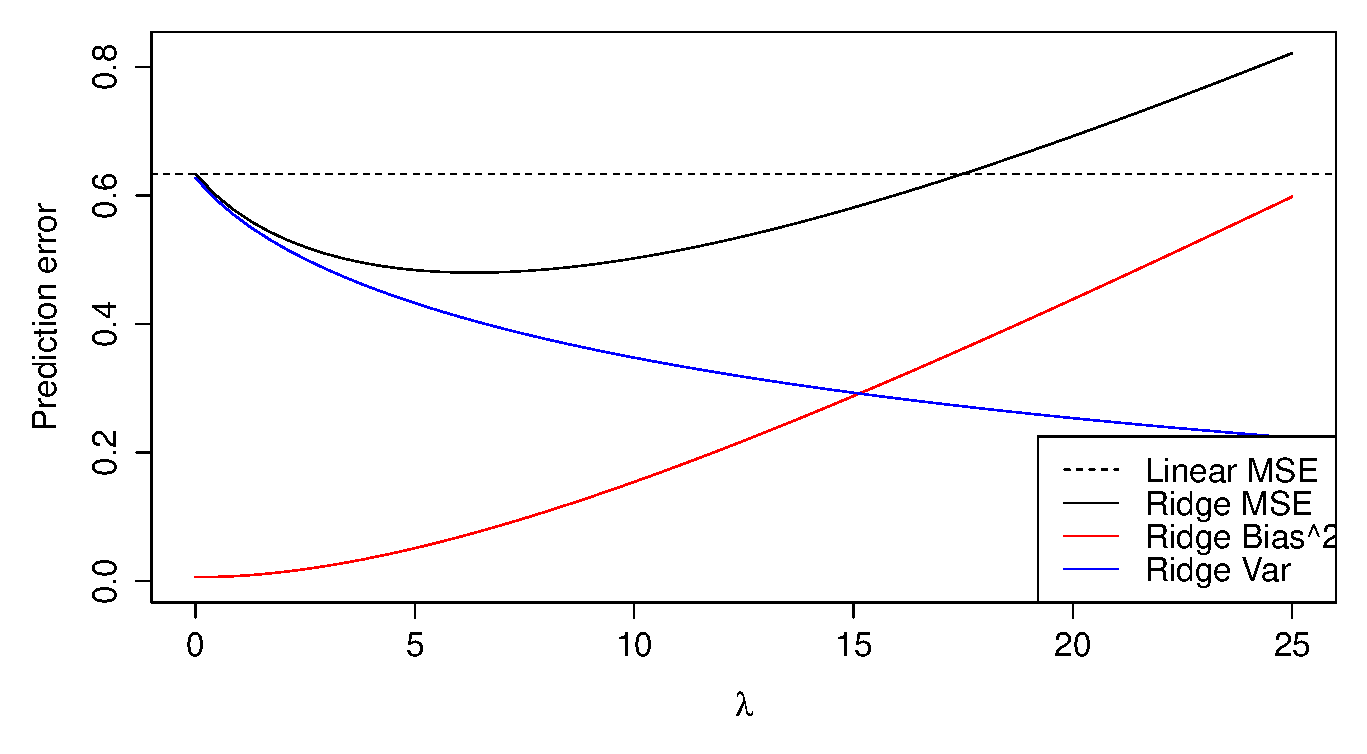
\includegraphics[width=0.8\linewidth]{plots/biasvariance}
\caption{Bias-variance tradeoff}
\label{fig:biasvariance}
\end{figure}

The figure~\ref{fig:biasvariance} shows the bias-variance tradeoff
given by equation~(\ref{eq:prederror}). Ridge regression shows an
increasing bias and a decreasing variance. Despite OLS has zero bias,
its variance is greater than ridge for small values of $\lambda$.
It can be shown that, in terms of prediction error, ridge (black line)
is lower than OLS (dotted line)~\cite{hoerl+kennard1970}.



\subsection{Selection of lambda}

Despite the bias-variance tradeoff provides a conceptual framework for
determining a good model, is not directly useful. Some popular methods
for determine model selection are:

\begin{itemize}
    \item Akaike information criterion (AIC) (Akaike, 1974)
    \item Bootstrap-based selection (Efron and Tibshirani, 1997)
    \item Cross-validation (Stone, 1974)
\end{itemize}

On the other hand, $\lambda$ can also be used to reduce computational time as it
is shown in equation~(\ref{eq:taylor}). Golub (~\cite{golub1965}) suggested that
$\lambda$ be chosen so that:

\[
\frac{\lambda}{\lambda + \delta^2} < 0.1
\]

\noindent where $\delta$ is a lower bound of the smallest non-zero singular
value $\sigma_k$. One approach is to choose the greatest lower bound for
$\delta=\sigma_k$. Hence:

\[
\frac{\lambda}{\lambda + \sigma_k^2} < 0.1
\]

\noindent if we choose $\lambda=\beta \sigma_k^2$ then we get the following
relation:


\[
\frac{\beta \sigma_k^2}{\beta \sigma_k^2 + \sigma_k^2} =
\frac{\beta}{\beta+1} < 0.1 \Rightarrow \beta < \frac{1}{9}  
\]

Experiments done by ~\cite{coleman+sun2010} have shown that $\beta = 0.01$
produces satisfactory results. This means that $\lambda = 0.01 \sigma_k^2$.

However, get $\sigma_k$ imply obtaining first the SVD, which is
computational expensive.

Since the algorithm presented by ~\cite{coleman+sun2010} already compute the QR
factorization of the matrix $\mathbf{A}$ they show a procedure for getting
a $\lambda$ approximation using QR.

\begin{enumerate}
\item Compute QR factorization: $\mathbf{A} = \mathbf{Q_1R_1}$
\item Let $\mathbf{W}$ denote the set of absolute values of the nonzero diagonal
elements of $\mathbf{R_1}$. Let $w_{\text{min}}$ and $w_{\text{max}}$ denote the
smallest and largest elements of $\mathbf{W}$ respectively. Both 
$\lambda_1 = \hat{\beta} w_{\text{min}}^2$
$\lambda_2 = \hat{\beta} \frac{w_{\text{min}}^2}{w_{\text{max}}^2}$ where
$\hat{\beta}=0.00025$ produce satisfactory results.
\item The $\lambda_{\text{QR}}$ approximation is obtained as:
$\lambda_{\text{QR}} = \frac{\lambda_1 + \lambda_2}{2}$  
\end{enumerate}

